\section{Derivazione dell'equazione del calore}
Definiamo innanzitutto le variabili in gioco:\\
$t=$ tempo, $x=$ posizione, $u(t,x)=$ temperatura nella posizione $x$ e al tempo $t$.\\
Nel definire il modello si far\`a uso di:
%
\begin{align*}
& r= \mbox{ tasso di calore per unit\`a di massa dall'esterno } \; [r]=\frac{[cal]}{[tempo][massa]}\\
& \rho= \mbox{ densit\`a (lineare) di massa della barra } \; [\rho]=\frac{[massa]}{[lunghezza]}\\
& q= \mbox{ flusso di calore } \; [q]=\frac{[cal]}{[tempo]}\\
& e= \mbox{ energia interna per unit\`a di massa } \; [r]=\frac{[cal]}{[massa]}\\
\end{align*}

Il primo passo nella derivazione dell'equazione del calore consiste
nell'applicare la \textit{Legge di Bilancio}:
isolata una porzione $[x_0, x_0+h]$ della barra, il tasso di variazione dell'energia interna eguaglia il flusso agli estremi;
nel caso di sorgente, il tasso di variazione del calore erogato sar\`a sommato al flusso agli estremi.
\[
	\underbrace{\frac{d}{dt}\int_{x_0}^{x_0+h} e(t,x)\rho
dx}_{\mathclap{\text{Variazione dell'energia rispetto al tempo}}}
	= \overbrace{q(t,x_0)-q(t,x_0 +h)}^\text{Flusso entrante}
	+\underbrace{\int_{x_0}^{x_0+h} r(t,x) \rho dx}_\text{Flusso della
sorgente}
\]
Per il Teorema Fondamentale del Calcolo Integrale
\[
	q(t,x_0)-q(t,x_0 +h) = -\int_{x_0}^{x_0+h} q_x(t,x)dx
\]
dove $q_x$ indica $\frac{dq}{dx}$.\\
Considerando che l'espressione
\[
	\frac{d}{dt}\int_{x_0}^{x_0+h} e(t,x)\rho dx
	= -\int_{x_0}^{x_0+h} q_x(t,x)dx
	+\int_{x_0}^{x_0+h} r(t,x) \rho dx
\]
deve essere valida per $x_0$ e $x_0+h$ e che, data la continuit\`a dell'energia
\`e possibile portare
la derivata all'interno del segno di integrale, si ottiene la Legge di Bilancio
in forma locale
\[
	\frac{\partial}{\partial t} e(t,x)\rho= -\frac{\partial}{\partial
x}q(t,x)+\rho r(t,x)
\]
\`E ora necessario applicare le leggi costitutive, che risultano essere delle
leggi sperimentali.\\
La prima, che prende il nome di \textit{Legge di Fourier}, indica che il flusso
di calore $q$ \`e direttamente proporzionale
alla derivata spaziale della temperatura secondo la legge
\[
	q= -ku_x
\]
con $u=u(t,x)$ e $k>0$. Il segno negativo indica che si ha il flusso positivo
passando dalla zona pi\`u calda a quella pi\`u fredda.
\[
	[k]= \frac{[cal]}{[tempo]}\frac{[lunghezza]}{[grado]}
\]
La seconda lega invece l'energia alla temperatura
\[
	e= c_lu
\]
dove $c_l$ indica il calore specifico ed \`e $>0$
\[
	[c_l]=\frac{[cal]}{[massa][grado]}
\]
Operando la sostituzione si ottiene
\[
	\rho c_l \frac{\partial}{\partial t} u= k \frac{\partial^2}{\partial
x^2}u + \rho r
\]
che riordinata
\[
	u_t= \underbracket{D}_{\mathclap{\text{Risposta termica}}} u_{xx}+f
\]
dove $D=k/(c_l\rho)$ e $f=r/c_l$.
\[
	[D]=\frac{\cancel{[cal]}[lunghezza]}{[tempo]\cancel{[grado]}}\frac{
\cancel{[massa]}\cancel{[grado]}}{\cancel{[cal]}}
	\frac{[lunghezza]}{\cancel{[massa]}}=\frac{[lunghezza]^2}{[tempo]}
\]
L'equazione caratteristica risulta quindi essere, considerata l'equazione
differenziale omogenea e sostituendo due variabili algebriche alle due variabili
derivate
\[
	u_t= Du_{xx} \;\;\; \Rightarrow \;\;\; T=DX^2
\]
Si noti che \`e l'equazione di una parabola.

%%%%%%%%%%%%%%%%%%%%%%%%%%%%%%%%%%%%%%%%%%%%%%%%%%%%%%%%%%%%%%%%%%%%%%%%%%%%%%%%
%%%%%%%%%%%%%%%%%%%%%%%%%%%
\section{Problemi ``Ben Posti''}
Si considerino i cosiddetti ``problemi ben posti'', essi saranno del tipo
\[
	\left\{
	\begin{array}{ll}
		u_t=Du_{xx} & x\in\mathbb{R}, \; 0<t<T \\
		u(0,x)=g(x) & \text{Temperatura Iniziale}\\
		u(t,0)=\alpha(t) \; , \; u(t,L)=\beta(t) & \text{Condizioni di
Dirichlet agli estremi}\\
		u_x(t,0)=\alpha(t) \; , \; u_x(t,L)=\beta(t) & \text{Condizioni
di Neumann agli estremi}
	\end{array}
	\right.
\]
Le condizioni di Dirichlet corrispondono a fissare la temperatura sui capi della
sbarra, mentre con Neumann si fissa
il flusso (condizioni di Neumann nulle significano che la barra \`e isolata agli
estremi). Non sono state poste condizioni per $t=T$
per la causalit\`a del sistema in esame.

\section{Unicit\`a e dipendenza continua dai dati}
Si inizia con il considerare la temperatura sulla barra
\[
	E(t)= \frac{1}{2}\int_0^L u^2 (t,x) dx
\]
e la si deriva rispetto al tempo
\[
	E'(t)= \frac{1}{2}\int_0^L 2u(t,x)u_t(t,x)dx
\]
Nel passaggio precedente ci si \`e posti nella condizione in cui la derivata
della somma equivale alla somma delle derivate.\\
Considerando ora $u_t=Du_{xx}$ si ottiene
\[
	E'(t)= D\int_0^L u(t,x)u_{xx}(t,x)dx
\]
Ora, utilizzando l'integrazione per parti
\[
	D\left[u(t,x)u_x(t,x)\right]_0^L - D\int_0^L
	\underbrace{u_x(t,x)u_x(t,x)}_{u_x^2(t,x)}dx
\]
Nel caso di condizioni agli estremi nulle si ha $u(t,0)=u(t,L)=0$, perci\`o il
termine $D\left[u(t,x)u_x(t,x)\right]_0^L=0$ e quindi
\[
	E'(t)= - D \int_0^L u_x^2(t,x) dx \leq 0
\]
La derivata negativa (o nulla) indica che $E(t)\leq E(0)$, segue che
\[
	\int_0^L u^2(t,x)dx \leq \int_0^L g^2 (x) dx
\]
Perci\`o, considerato il sistema privo di ingressi e quindi l'equazione
omogenea, $E(t)$ non aumenta. \\
Si consideri nuovamente l'equazione $u_t=Du_{xx}$; essa \`e lineare, perci\`o
se $u_1$ e $u_2$ sono soluzioni e $C_1,\; C_2$ costanti, anche $u=C_1u_1+C_2u_2$
\`e soluzione.\\
Se
\[
	\underbracket{
		\begin{array}{l}
			u_1 \text{ \`e soluzione con temperatura iniziale } g_1
\\
			u_2 \text{ \`e soluzione con temperatura iniziale } g_2
		\end{array}
		}_{\Downarrow}
\]
\[
	u_1-u_2 \text{ \`e soluzione con temperatura iniziale } g_1-g_2
\]
e applicato alla disuguaglianza precedente
\[
	\int_0^L \left(u_1(t,x)-u_2(t,x)\right)^2 dx
	\leq
	\int_0^L \left(g_1(x)-g_2(x)\right)^2 dx
\]
che garantisce:\\
{\bf Unicit\`a}: Se $g_1=g_2$ si ottiene
\[
	\int_0^L \underbrace{\left(u_1(t,x)-u_2(t,x)\right)^2}_\text{sempre
positivo o nullo} dx
	\leq 0
\]
essendo la somma di quadrati sempre positiva
\[
	\int_0^L \left(u_1(t,x)-u_2(t,x)\right)^2 dx
	= 0
\]
e quindi $u_1(t,x)=u_2(t,x)$
Perci\`o con le stesse condizioni iniziali si ottiene la stessa soluzione.\\
{\bf Dipendenza continua della soluzione dai dati}:\\
Una differenza infinitesima nelle condizioni iniziali comporta una differenza
infinitesima nella soluzione, garantendo la continuit\`a dai dati (non diverge).

\section{Problema di Cauchy globale}
Riprendendo il problema di Dirichlet con condizioni nulle agli estremi
\[
	\left\{
	\begin{array}{l}
		u_t=Du_{xx} \\
		u(0,x)=g(x) \\
		u(t,0)=0, \; u(t,L)=0
	\end{array}
	\right.
\]
Svincoliamo ora la soluzione da $g(x)$ (sar\`a ripreso successivamente)
\[
	\left\{
	\begin{array}{l}
		u_t=Du_{xx} \\
		u(t,0)=0, \; u(t,L)=0
	\end{array}
	\right.
\]
Procediamo poi utilizzando la tecnica della separazione delle variabili.\\
Si consideri $u(t,x)=v(t)w(x)$, perci\`o
\[
	\left\{
	\begin{array}{l}
		v'(t)w(x)=Dv(t)w''(x) \\
		w(0)=w(L)=0
	\end{array}
	\right.
\]
dividendo per $v(t)w(x)$ si ottiene
\[
	\left\{
	\begin{array}{l}
		\displaystyle{\frac{v'(t)}{v(t)}=D\frac{w''(x)}{w(x)} }\\
		w(0)=w(L)=0
	\end{array}
	\right.
\]
Essendo le variabili di integrazione diverse, equivale a dire
\[
	\frac{v'(t)}{v(t)}=K=D\frac{w''(x)}{w(x)}
\]
con $K$ una costante. Perci\`o si possono spezzare in due equazioni
\[
	\left\{
	\begin{array}{l}
		\displaystyle{D w''(x) - Kw(x) = 0 }\\
		w(0)=w(L)=0
	\end{array}
	\right.
	\;\;\;
	\text{ e }
	\;\;\;
	v'(t)=Kv(t)
\]
Procediamo con il risolvere l'equazione differenziale di secondo grado;
essa imporr\`a dei vincoli su $K$.
\[
	D\lambda^2-K=0
\]
\[
	\lambda^2=\frac{K}{D}
\]
Si distinguono ora i vari casi:
\begin{itemize}
	\item $K>0$
	\item $K=0$
	\item $K<0$
\end{itemize}

{\bf Se $K>0$}:
\[
	\lambda=\pm \sqrt{\frac{K}{D}}
\]
\[
	w(x)= C_1e^{x\sqrt{\frac{K}{D}}} + C_2e^{-x\sqrt{\frac{K}{D}}}
\]
applicando le condizioni al contorno ($w(0)=0 \; w(L)=0$)
\[
	\left\{
	\begin{array}{l}
		C_1+C_2=0 \\
		\displaystyle{C_1e^{L\sqrt{\frac{K}{D}}}
			+ C_2e^{-L\sqrt{\frac{K}{D}}}}
	\end{array}
	\right.
	\;\;\;
	\Rightarrow
	\;\;\;
	\left\{
	\begin{array}{l}
		C_1=0\\
		C_2=0
	\end{array}
	\right.
\]
Perci\`o l'insieme delle soluzioni con $K>0$ verr\`a scartato.

{\bf Se $K=0$}:
\[
	w''=0
	\;\;\;
	\Rightarrow
	\;\;\;
	w(x)=C_1x + C_2
\]
\[
	\left\{
	\begin{array}{l}
		w(x)=C_1x + C_2\\
		w(0)=0, \; w(L)=0
	\end{array}
	\right.
	\;\;\;
	\Rightarrow
	\;\;\;
	\left\{
	\begin{array}{l}
		C_1=0\\
		C_2=0
	\end{array}
	\right.
\]
Anche la soluzione con $K=0$ sar\`a scartata.

{\bf Se $K<0$}:\\
Poniamo $-\omega^2 = K/D$ $\Rightarrow$ $\lambda^2 = - \omega^2$ e $\lambda=\pm
i\omega$
\[
	\left\{
	\begin{array}{l}
		w(x)=C_1 cos(\omega x) + C_2 sin(\omega x)\\
		w(0)=0, \; w(L)=0
	\end{array}
	\right.
	\;\;\;
	\Rightarrow
	\;\;\;
	\left\{
	\begin{array}{l}
		C_1=0\\
		C_2 sin(\omega L)= 0
	\end{array}
	\right.
\]
\[
	\sin (\omega L)=0
	\;\;\;
	\Rightarrow
	\;\;\;
	\omega L = n\pi
	\;\;\;
	\Rightarrow
	\;\;\;
	\omega_n= \omega= n \frac{\pi}{L} \text{, con }n=1,2,3,\ldots
\]
Ora, considerata la soluzione n-esima di $w(x)$
\[
	w_n(x)=sin\left(\frac{n\pi}{L}x \right)
\]
dove la costante $C_2$ sar\`a considerata successivamente, al momento della
scomposizione con Fourier.\\
Considerato ora
\[
	K_n=-\omega_n^2 D= -\left(\frac{n\pi}{L}\right)^2D
\]
procediamo con il risolvere l'equazione differenziale di primo grado
\[
	v'(t)= Kv(t)
\]
\[
	v_n(t)= e^{Kt}=e^{-\left(\frac{n\pi}{L}\right)^2Dt}
\]
Riprendendo  $u_n(t,x)= w_n(x) v_n(t)$ si ottengono le infinite soluzioni
di base del problema di Dirichlet iniziale
\[
	u_n(t,x)= e^{-\frac{n^2\pi^2}{L^2} Dt}
	sin\left(\frac{n\pi}{L}x \right)
\]
A questo punto Fourier considera la possibilit\`a di scomporre qualsiasi
soluzione come serie di sinusoidi, quindi
\[
	u= \sum_{n=1}^{\infty} b_n u_n(t,n)=
	\sum_{n=1}^{\infty}b_n e^{-\frac{n^2\pi^2}{L^2} Dt}
	sin\left(\frac{n\pi}{L}x \right)
\]
dove i vari $b_n$ rappresenterebbero i precedenti $C_{2(n)}$.\\
A questo punto \`e possibile definire anche le condizioni con $t=0$ attraverso
la scomposizione in \textit{serie di Fourier}, infatti $u(0,x)=g(x)$, perci\`o
\[
	g(x)= \sum_{n=1}^{\infty} b_n sin\left(\frac{n\pi}{L}x \right)
\]
con $0\leq x \leq L$.\\
Bisogna quindi trovare un modo per poter esprimere la funzione $g(x)$
come serie di sinusoidi.\\
Verifichiamo prima di tutto la convergenza.\\
Si prenda una sequenza limitata dei coefficienti $b_n$, tale che
$|b_n|\leq C$ per qualsiasi $n$, data $C$ una costante. Allora se $t \geq t_0 >
0$
e $0\leq x \leq L$
\[
	\sum_{n=1}^{\infty}\left| b_n e^{-\frac{n^2\pi^2}{L^2} Dt}
	sin\left(\frac{n\pi}{L}x \right)\right|
	\leq
	\sum_{n=1}^{\infty}\left| b_n \right| e^{-\frac{n^2\pi^2}{L^2} Dt}
	\leq
	C \underbrace{\sum_{n=1}^{\infty}e^{-\frac{n^2\pi^2}{L^2} Dt}}
	_\text{Serie convergente}
\]
Siccome ogni addendo \`e soluzione dell'equazione, se risulta possibile
derivare all'interno della serie, anch'essa \`e soluzione. Questo pu\`o essere
effettuato nel caso in cui la somma della serie converga.
\[
	\sum_{n=1}^{\infty}\left| \frac{\partial}{\partial x} u_n \right|=
	\sum_{n=1}^{\infty}\left| b_n \frac{n\pi}{L}
	e^{-\frac{n^2\pi^2}{L^2} Dt}
	sin\left(\frac{n\pi}{L}x \right)\right|
	\leq
	C \sum_{n=1}^{\infty} \frac{n\pi}{L} e^{-\frac{n^2\pi^2}{L^2} Dt}
\]
In questo caso $e^{-n^2}$ tende a zero molto rapidamente, rendendo la serie
convergente. Successivamente anche la derivata seconda converge
(in realt\`a \`e una funzione liscia, cio\`e $u(t,x)\in C^\infty$,
per $t>0$ e $0\leq x \leq L$).
Qualunque sia $g(x)$, passato l'istante $t=0$, la funzione diventa
immediatamente
continua. La diffusione ha quindi un effetto regolarizzante.\\
\`E quindi possibile derivare all'interno della sommatoria.\\
Si tratta ora di costruire il prolungamento dispari con periodo $2L$ (fig.
\ref{prolper_disp})
\begin{figure}[H]
	\centering
	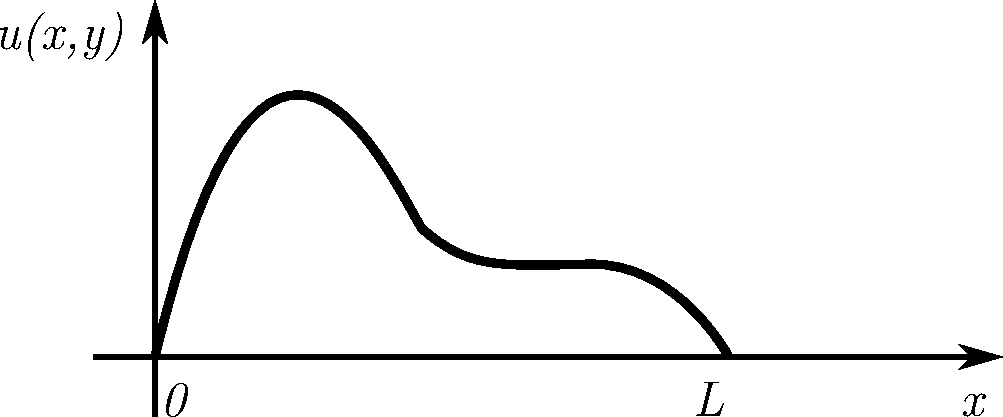
\includegraphics[width=0.5\textwidth]{gx.pdf}
	\caption{Funzione $g(x)$.}
	\label{gx}
\end{figure}
\begin{figure}[H]
	\centering
	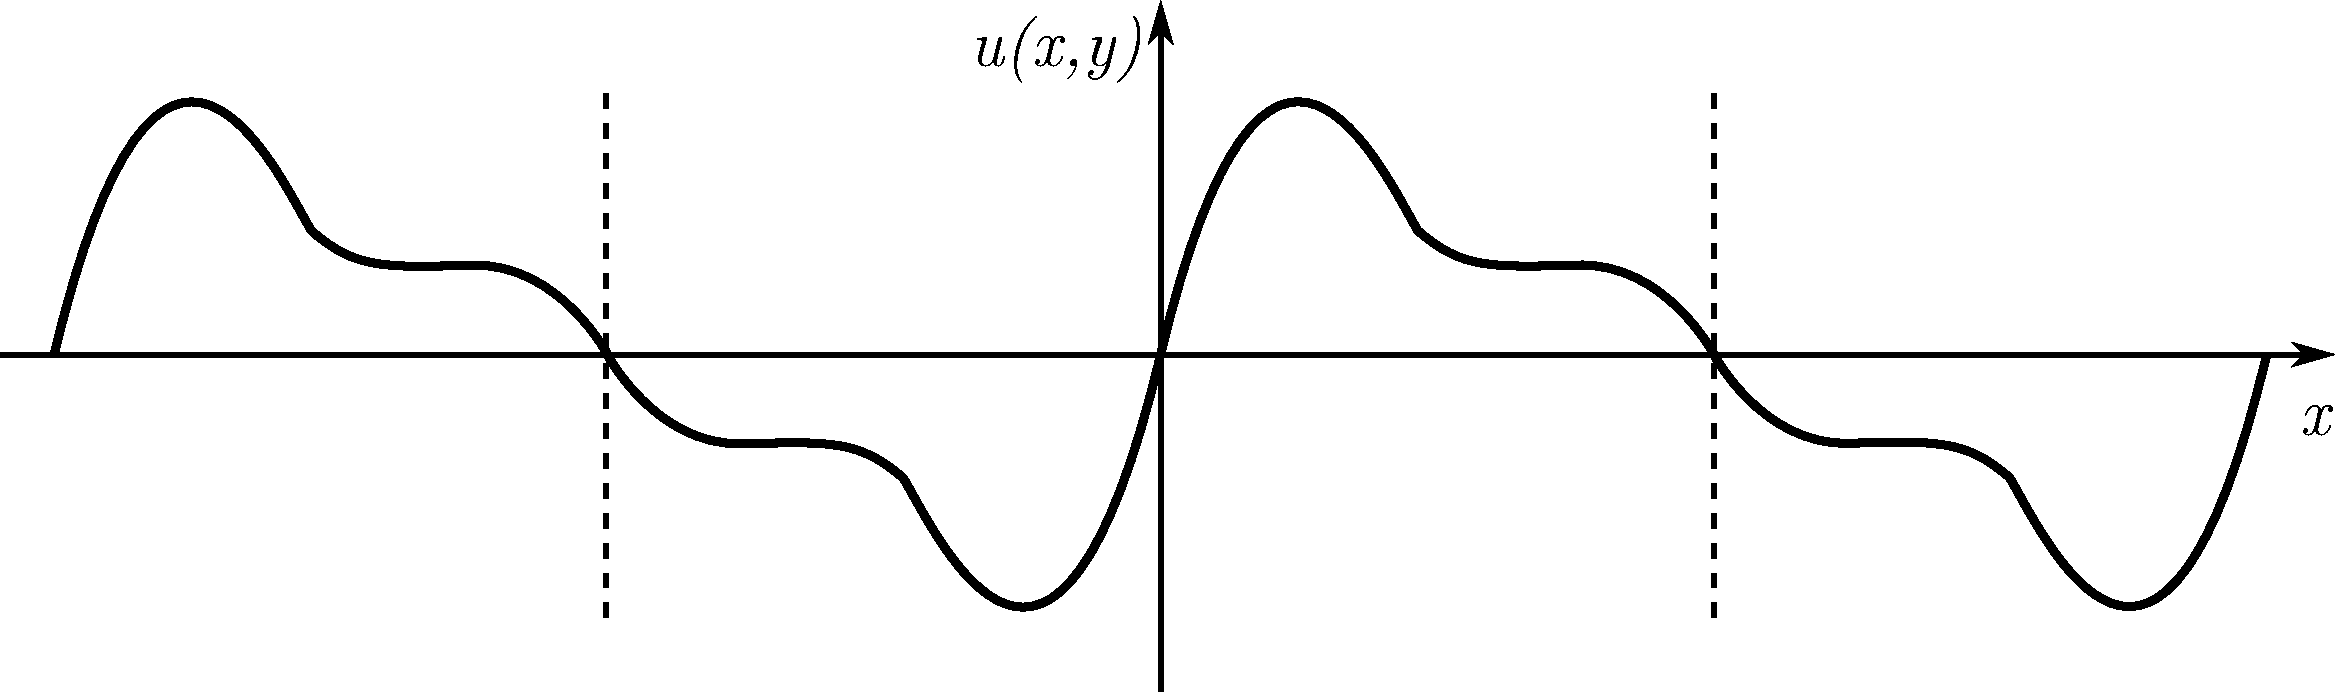
\includegraphics[width=\textwidth]{prolper_disp.pdf}
	\caption{Prolungamento periodico dispari.}
	\label{prolper_disp}
\end{figure}
\noindent
Si \`e operato con un prolungamento dispari in modo da ottenere una serie
composta
da sole sinusoidi. Si noti che nella parte di interesse, cio\`e tra $0$ e $L$,
rappresenta effettivamente la funzione $g(x)$.
\[
	b_n= \frac{2}{L}\int_0^L g(x)sin \left(\frac{n\pi}{l} x\right) dx
	\;\;\; \text{con} \;\;\;
	\omega= \frac{2\pi}{2L}= \frac{\pi}{L}
\]
Ricavati i $b_n$ \`e possibile ottenere la funzione $u(x,t)$.

Il coefficiente di scala \`e dato da $D/L^2$; questo consente di
scalare le dimensioni variando opportunamente il materiale, rendendo possibile
l'uso di modellini equivalenti (scalati).
\[
	\frac{D_1}{L_1^2}= \frac{D_2}{L_2^2}
\]
\subsection{Esercizio: Condizioni agli estremi non nulle}
\[
	\left\{
	\begin{array}{l}
		u_t=Du_{xx} \\
		u(0,x)=g(x) \\
		u(t,0)=\theta_1 \\
		u(t,L)=\theta_2
	\end{array}
	\right.
\]
con $\theta_1 \neq \theta_2$.\\
Si inizia con il considerare una soluzione stazionaria del problema, cio\`e
indipendente dal tempo
\[
	\left\{
	\begin{array}{l}
		\cancel{u_t}=Du_{xx}^S \\
		u(0,x)=g(x) \\
		u^S(\cancel{t},0)=\theta_1 \\
		u^S(\cancel{t},L)=\theta_2
	\end{array}
	\right.
	\;\;\;
	\Rightarrow
	\;\;\;
	\left\{
	\begin{array}{l}
		Du_{xx}^S= 0 \\
		u(0,x)=g(x) \\
		u^S(0)=\theta_1 \\
		u^S(L)=\theta_2
	\end{array}
	\right.
\]
\[
	(u^S)''(x)=0 \;\;\; \Rightarrow \;\;\; u^S(x)=ax+b
\]
\[
	u^S(0)= \theta_1 \;\;\; \Rightarrow \;\;\; b= \theta_1
\]
\[
	u^S(L)= \theta_2 \;\;\; \Rightarrow \;\;\; aL+\theta_1= \theta_2
	\;\;\; \Rightarrow \; \; \; a= \frac{\theta_2 - \theta_1}{L}
\]
\begin{figure}[H]
	\centering
	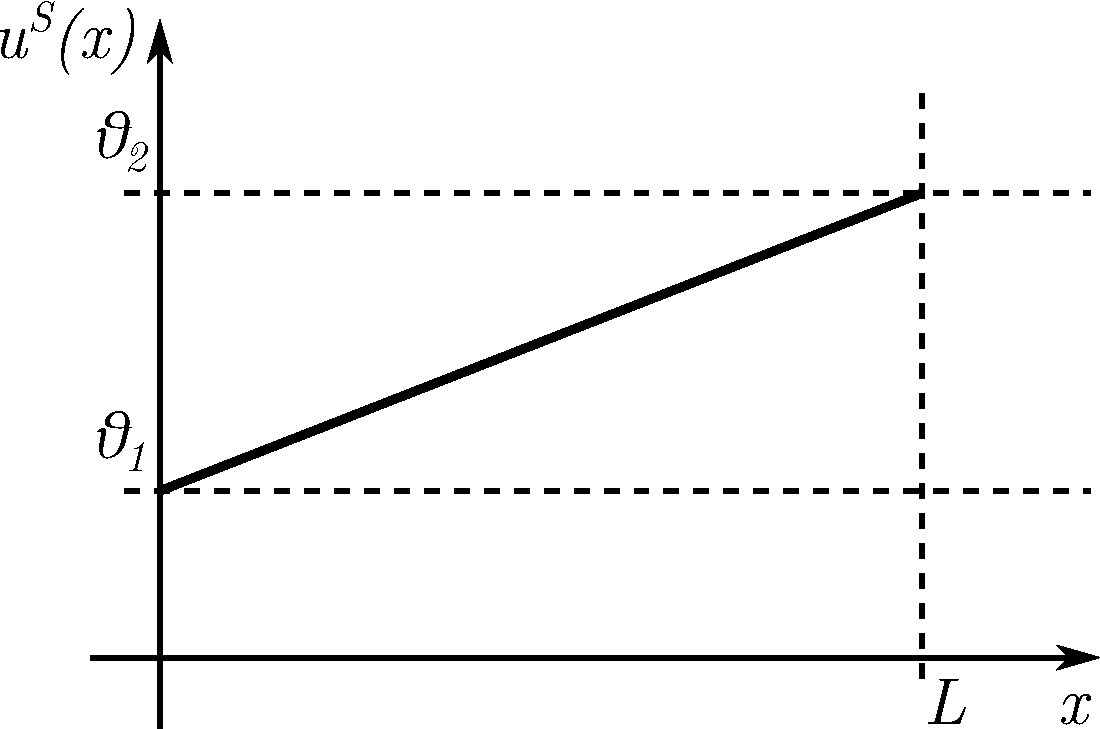
\includegraphics[width=0.5\textwidth]{nonomog_stationary.pdf}
	\caption{Soluzione stazionaria.}
	\label{nonomog_stationary}
\end{figure}
La soluzione \`e composta quindi dalla soluzione stazionaria e dalla soluzione
con condizioni agli estremi nulle.
\[
	u(t,x)= \underbrace{v(t,x)}_{\mathclap{\text{Transitorio}}} + u^S(x)
\]
con $u(0,x)= v(0,x) + u^S(x) \;\;\; \Rightarrow \;\;\; v(0,x)=g(x)- u^S(x)$
\[
	\left\{
	\begin{array}{l}
		v_t=Dv_{xx} \\
		v(0,x)=g(x)- u^S(x) \\
		v(t,0)=0 \\
		v(t,L)=0
	\end{array}
	\right.
\]
\subsection{Esercizio: Barra isolata agli estremi}
\[
	\left\{
	\begin{array}{l}
		u_t=Du_{xx} \\
		u(0,x)=g(x) \\
		u_x(t,0)=0 \\
		u_x(t,L)=0
	\end{array}
	\right.
\]
Si ottiene che la soluzione \`e composta da una serie di soli coseni a
valor medio non nullo
\[
	u(t,x)= \frac{a_0}{2}+ \sum_{n=1}^\infty a_n
	e^{-\frac{n^2\pi^2}{L^2} Dt}
	cos \left(\frac{n\pi}{L}x \right)
\]
\[
	\frac{a_0}{2}= \frac{1}{L}\int_0^L g(x)dx
\]
\begin{figure}[H]
	\centering
	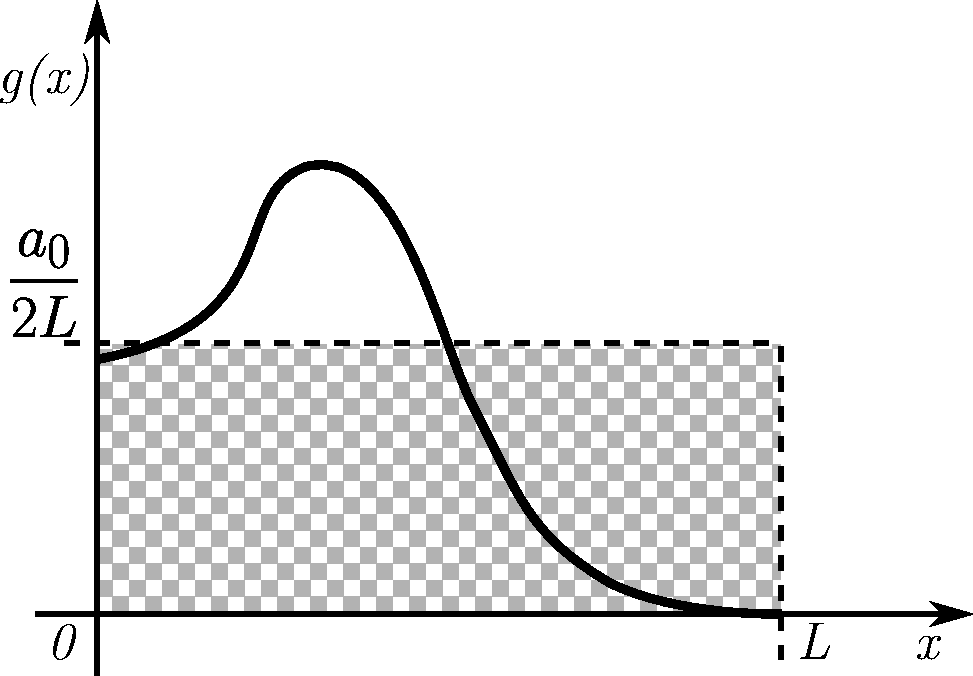
\includegraphics[width=0.5\textwidth]{isol_bar.pdf}
	\caption{Valor medio di $g(x)$ con barra isolata.}
	\label{isol_bar}
\end{figure}
%%%%%%%%%%%%%%%%%%%%%%%%%%%%%%%%%%%%%%%%%%%%%%%%%%%%%%%%%%%%%%%%%%%%%%
\section{Barra con lunghezza infinita}
\[
	\left\{
	\begin{array}{ll}
		u_t=Du_{xx} \\
		u(0,x)=g(x) & -\infty < x < \infty \\
	\end{array}
	\right.
\]
Il comportamento agli estremi ($-\infty < x < \infty$) \`e inglobato nella
definizione dello spazio al quale deve appartenere la soluzione.
\subsection{Soluzione fondamentale}
La soluzione fondamentale descrive la diffusione per $t>0$ di una massa unitaria
concentrata in $x=0$ al tempo $t=0$. Questo significa
\[
	\left\{
	\begin{array}{l}
		u_t=Du_{xx}, \;\;\; t>0 \\
		u(0,x)= \delta(x)  \\
	\end{array}
	\right.
\]
Si utilizzer\`a la trasformata di Fourier rispetto ad $x$ di $u(x,t)$ definita
da
\[
	v(t,\lambda)=\int_{-\infty}^{+\infty} e^{-i\lambda x} u(t,x) dx
\]
nel caso che $u(t,x)$ sia sommabile da $- \infty$ a $+ \infty$ in $dx$ per
$t>0$. Ricordiamo che la trasformata si estende a distribuzioni di Schwartz
di cui anche $\delta (x)$ fa parte, con trasformata pari a $1$.
Allora \`e equivalente a
\[
	\left\{
	\begin{array}{l}
		v_t=D\left( i\lambda \right)^2 v \;\; = -D\lambda^2 v\\
		v(0,\lambda)= 1  \\
	\end{array}
	\right.
\]
con $\hat{\delta}= 1$ e $\partial_x \Leftrightarrow i\lambda$.\\
L'integrale generale dell'equazione vale
\[
	v(t,\lambda)= C(\lambda)e^{-D\lambda^2 t}
\]
che fissate le condizioni agli estremi
\[
\begin{array}{c}
	v(0,t)= 1 \;\;\; \Rightarrow \;\;\; c(\lambda)= 1\\
	\Downarrow \\
	v(t,\lambda)= e^{-D\lambda^2 t}
\end{array}
\]
Si tratta di una trasformata notevole
\[
	u(t,x)= \frac{1}{\sqrt{4 \pi D t}}
	e^{-\frac{x^2}{4Dt}}
\]
Questa \`e l'unica soluzione di
\[
	\left\{
	\begin{array}{l}
		u_t=Du_{xx}, \;\;\; t>0 \\
		u(0,x)= \delta(x)  \\
	\end{array}
	\right.
\]
tale che $u(t, \bullet) \in \mathcal{S'}, \;\; t \geq 0$.
\begin{figure}[H]
	\centering
	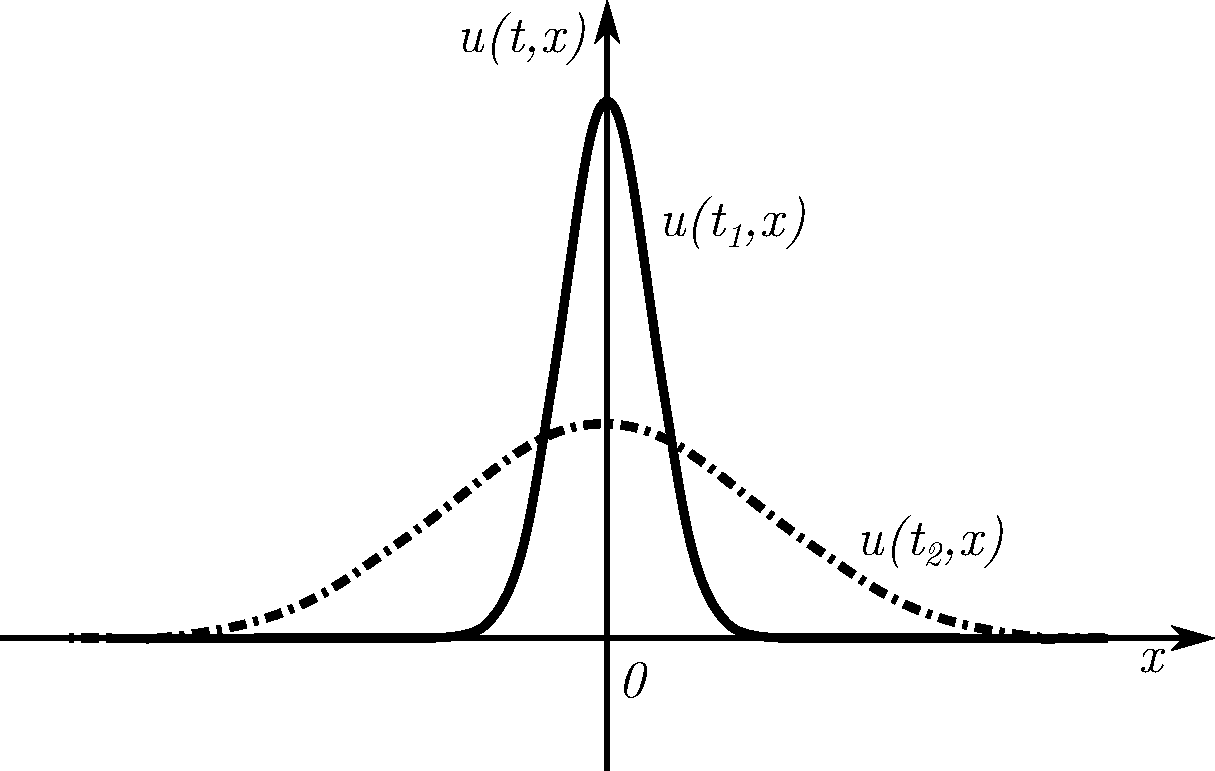
\includegraphics[width=0.8\textwidth]{gauss_bell.pdf}
	\caption{$u(t,x)$ con $t_1$, $t_2$ fissati tali che $t_2>t_1>0$.}
	\label{gauss_bell}
\end{figure}
Il fatto che,
\[
	\intR u(t,x) dx =
	\frac{1}{\sqrt{4 \pi D t}}
	\intR e^{-\frac{x^2}{4Dt}} dx
\]
operando le sostituzioni,
\[
\frac{x}{\sqrt{4Dt}}= y \;\;\; \text{e} \;\;\; \frac{dx}{\sqrt{4Dt}}= dy
\]
\[
	\frac{1}{\sqrt{\pi}}\intR e^{-y^2} dy= \frac{1}{\sqrt{\pi}}\sqrt{\pi}=1
\]
esprime la conservazione della massa totale ad ogni tempo $t>0$.
La massa unitaria inizialmente centrata nel punto $x=0$ si diffonde con
densit\`a gaussiana di scarto quadratico $4Dt$ al tempo $t$ (fig.
\ref{gauss_bell}).
\subsection{Trasformazioni invarianti}
\subsubsection{Traslazione temporale}
Consideriamo una soluzione $u(t,x)$ di
\[
	u_t= Du_{xx} \;\;\; 0< t< T, \;\;\; - \infty <x < +\infty
\]
La funzione
\[
	v(t,x)= u(T-t,x)
\]
\`e tale che
\[
	v_t(t,x)= -u_t(T-t, x)
\]
\[
	v_{xx}(t, x)= u_{xx}(T-t,x)
\]
quindi risolve l'equazione
\[
	v_t= -Dv_{xx}
\]
La non invarianza dell'equazione rispetto alla trasformazione $t \Rightarrow
T-t$
riflette la non reversibilit\`a temporale dei fenomeni di diffusione.
Il problema di Cauchy globale \`e ben posto con condizione iniziale al tempo
$t=0$ e nessuna condizione pu\`o essere posta al tempo finale $t=T$, in quanto
il comportamento nel futuro \`e completamente determinato dalla storia passata
(principio di causalit\`a).
Il problema
\[
	v_t= -Dv_{xx}
\]
\`e ben posto con la condizione al tempo $t=T$ e nessuna condizione pu\`o essere
posta al tempo $t=0$
\subsubsection{Invarianti di scala}
La trasformazione
\[
	t\Rightarrow at, \;\;\; x \Rightarrow bx, \;\;\; u\Rightarrow cu,
	\;\;\;
	\text{ con }
	a,b,c>0
\]
\`e un cambio di scala (omotetia) per il grafico di $u$.

Vediamo sotto quali condizioni la funzione
\[
	v(t,x)= cu(at, bx)
\]
\`e ancora soluzione.
\[
	\begin{array}{l}
		v_t= acu_t \\
		v_{xx}= b^2 c u_{xx}  \\
		v_t= Dv_{xx} \\
		\left( u_t= Du_{xx} \right)
	\end{array}
\]
\[
	\Downarrow
\]
\[
	acu_t= Db^2 c u_{xx} \follows a=b^2
\]
Per ottenere il coefficiente $c$, prendiamo il esame la conservazione della
massa
\[
	\intR v(t,x) dx = \intR u(t,x) dx = m= 1
\]
perci\`o
\[
	\intR v(t,x) dx=
	\intR cu(at, \sqrt{a}x) dx= \frac{c}{\sqrt{a}}
	\intR u(at,y)
\]
sostituendo
\[
	y=\sqrt{a}x, \;\;\; dx= \frac{1}{\sqrt{a}}dy
\]
si ottiene
\[
	\frac{c}{\sqrt{a}}
	\intR u(at,y)dy= \frac{c}{\sqrt{a}}
	\follows
	\frac{c}{\sqrt{a}=1}
	\follows
	c=\sqrt{a}
\]
In conclusione
\[
	v(t,x)= \sqrt{a}u(at, \sqrt{a}x)
\]
\`e ancora una soluzione con la stessa massa totale conservata ad ogni $t>0$.\\
Le trasformazioni del tipo
\[
	t\Rightarrow at, \;\;\; x=\sqrt{a} x
\]
si chiamano dilatazioni paraboliche, in quanto lasciano invariati i rapporti
\[
	\frac{x^2}{t}, \;\;\; \frac{x}{\sqrt{t}}
\]
\section{Soluzione fondamentale senza l'uso della trasformata di Fourier}
Prendo formalmente $a= 1/t$ nelle dilatazioni paraboliche e cerchiamo una
soluzione
\[
	u^*(t,x)= \frac{1}{\sqrt{t}}u \left( 1, \frac{x}{\sqrt{t}} \right)=
	\frac{1}{\sqrt{t}}U \left( r \right)
\]
a variabili separate, come prodotto della funzione dl solo tempo
$\frac{1}{\sqrt{t}}$ e della funzione $U(r)$, da determinarsi, della sola
variabile
$r=\frac{x}{\sqrt{t}}$
\[
	u^*_t= -\frac{1}{2}t^{-\frac{3}{2}} U(r)
	+ t^{-\frac{1}{2}}U'(r) x \left( -\frac{1}{2}t^{-\frac{3}{2}} \right)
	= -\frac{1}{2}t^{-\frac{3}{2}} \left( U(r)+ rU'(r) \right)
\]
\[
	u^*_x= t^{-\frac{1}{2}}U'(r)t^{-\frac{1}{2}}=
	t^{-1} U'(r)
\]
\[
	u^*_{xx}=t^{-1}U''(r)t^{\frac{1}{2}}=
	t^{-\frac{3}{2}}U''(r)
\]
Considerando quindi
\[
	u^*_t=Du^x_{xx}
\]
ottengo
\[
	-\frac{1}{2} U(r) -\frac{1}{2}rU'(r)= DU''(r)
\]
\[
	2DU''(r)+ rU'(r)+ U(r)= 0
\]
che risulta essere una equazione differenziale a coefficienti non costanti.
I polinomi di grado finito non possono risolvere l'equazione, ma serve una
serie.
Cerchiamo le soluzioni come serie di potenze
\[
	U(r)= \sum_{n=0}^{\infty}a_n r^n
\]
\[
	U'(r)= \sum_{n=1}^{\infty} n a_n r^{n-1}
	= \sum_{n=0}^{\infty} n a_n r^{n-1}
\]
\[
	rU'(r)= \sum_{n=0}^{\infty} na_n r^n
\]
\[
	U''(r)=\sum_{n=2}^{\infty} n(n-1)a_n r^{n-2}
\]
sostituendo con la variabile d'appoggio $m=n-2$
\[
	U''(r)=\sum_{m=2}^{\infty} (m+2)(m+1)a_(m+2) r^{m}
\]
quindi richiamando l'indice $n$
\[
	U''(r)=\sum_{n=2}^{\infty} (n+2)(n+1)a_(n+2) r^{n}
\]
Sostituendo nell'equazione ed eguagliando a zero il coefficiente di $r^n$ per
ogni $k \geq $, si ha
\[
	2D(n+2)(n+1)a_{n+2}+ na_n+ a_n = 0
\]
\[
	2D(n+2)\cancel{(n+1)}a_{n+2}+ \cancel{(n+1)}a_n=0
\]
con $n+1 \neq 0$, ma $n$ parte da zero, perci\`o \`e sempre positivo.\\
La formula ricorsiva
\[
	a_{n+2}= -\frac{a_n}{2D(n+2)}
\]
fornisce tutti i coefficienti di indice pari, assegnato $a_0$, e tutti quelli
dispari assegnato $a_1$.
Del resto sappiamo che l'integrale generale dipende da due costanti arbitrarie.
Se siamo alla ricerca di una soluzione che descriva la diffusione di una massa
inizialmente concentrata in $x=0$, \`e naturale assumere che la densit\`a abbia
simmetria pari per $t>0$, perci\`o $a_1=0$ e quindi tutti gli $a$ con indice
dispari sono nulli.
Stabiliti $a_0$ e $a_1$ si \`e stabilita tutta la serie, con $n\rightarrow
\infty$.\\
Per quanto riguarda i coefficienti pari
\begin{align*}
	& a_0=\ldots \\
	& a_2= - \frac{1}{4D} a_0 \\
	& a_4= - \frac{1}{4D \cdot 2} a_2 = \left( -\frac{1}{4D} \right)^2
	\frac{1}{2} a_0 \\
	& a_6= - \frac{1}{4D \cdot 3} a_4 = \left( -\frac{1}{4D} \right)^3
	\frac{1}{3 \cdot 2} a_0 \\
	& a_{2(m+1)}= \left( -\frac{1}{4D} \right)^{m+1}
	\frac{1}{(m+1)!} a_0 \\
	& \text{sostituendo }m \rightarrow m+1 \\
	& a_{2m}= \left( -\frac{1}{4D} \right)^{m}
	\frac{1}{m!} a_0 \\
\end{align*}
Questa comprende anche $a_0$, infatti $a_0= 1 \cdot 1/1 \cdot a_0= a_0$\\
Riprendendo $U(r)$
\[
	U(r)= a_0 \sum_{m=0}^{\infty} \frac{1}{m!}
	\left( -\frac{1}{4D} \right)^m r^{2m}
	= a_0 \sum_{m=0}^{\infty} \frac{1}{m!}
	\left( -\frac{r^2}{4D} \right)^m
	= a_0 e^{- \left( r^2/4D \right)}
\]
dove si \`e usata la definizione attraverso la serie di potenze
dell'esponenziale
\[
	\sum_{m=0}^{\infty} \frac{x^m}{m!}= e^x
\]
Si sono quindi ottenute le soluzioni
\[
	u^*(t,x)= \frac{1}{\sqrt{t}}U(r)= \frac{a_0}{\sqrt{t}}
	e^{- \left( r^2/4D \right)}
	= \frac{a_0}{\sqrt{t}} e^{- \left( x^2/4Dt \right)}
\]
Imponendo che la massa conservata sia $m=1$, si ha
\[
	\intR u^*(t,x) dx= \frac{a_0}{\sqrt{t}}
	\intR e^{-\left( x^2/4Dt \right)} dx
\]
ponendo $x= \sqrt{4Dt}y$ e $dx= \sqrt{4Dt} dy$
\[
	\intR e^{-y^2}dy= \sqrt{\pi}
\]
perci\`o
\[
	\frac{a_0}{\sqrt{t}}\sqrt{4Dt}\sqrt{\pi}=a_0\sqrt{4D\pi}=1
\]
\[
	a_0= \frac{1}{\sqrt{4D\pi}}
\]
\[
	u^*(t,x)= u(t,x)= \frac{1}{\sqrt{4D\pi t}}
	e^{-\left( x^2/4Dt \right)}
	= \Gamma_D(t,x)
\]
con $t>0$. L'effetto \`e quindi quello gi\`a indicato in fig. \ref{gauss_bell}.
L'andamento di $\Gamma_D(t,x)$ per $t \rightarrow 0$ \`e uno dei fenomeni che
ha portato alla definizione della \textit{Delta di Dirac}.
Se lo scarto quadratico $4Dt \rightarrow 0$, la massa totale $m=1$ tende
a concentrarsi nel valor medio $x=0$.
\begin{figure}[H]
	\centering
	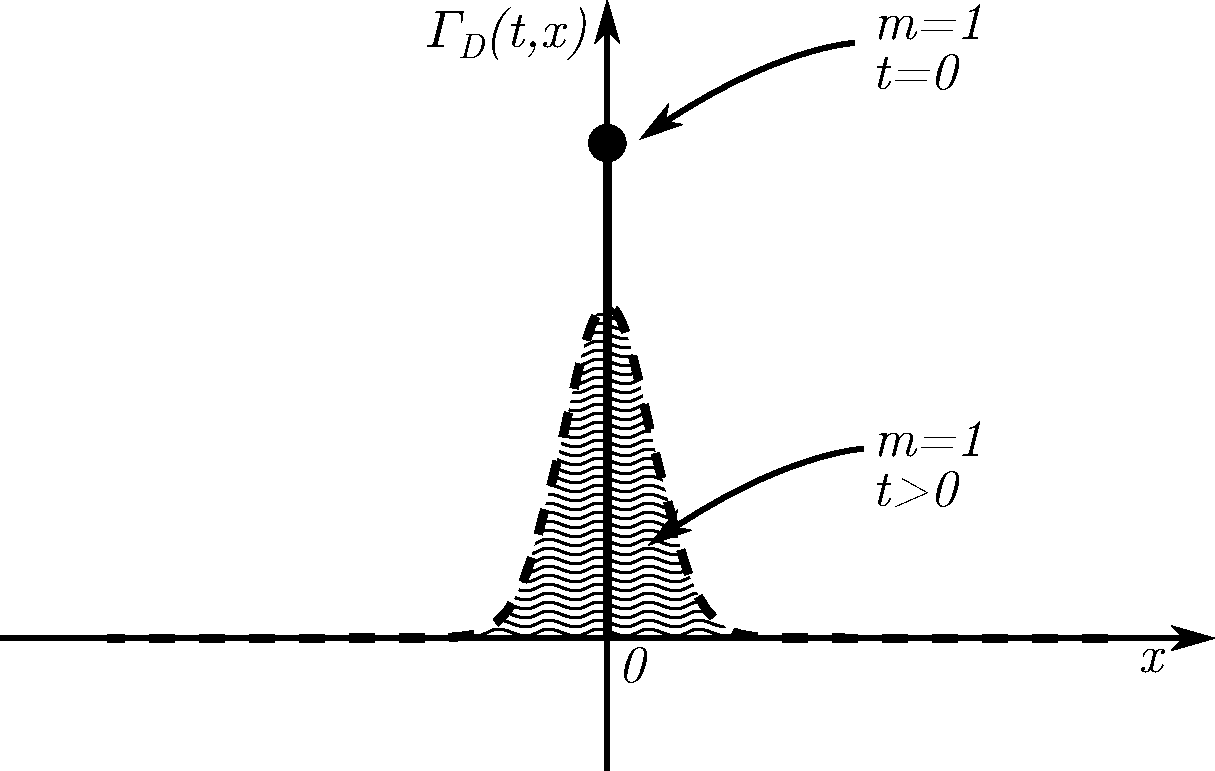
\includegraphics[width=0.8\textwidth]{gauss_bell_delta.pdf}
	\caption{La massa resta costante al variare di $t$.}
	\label{gauss_bell_delta}
\end{figure}
\noindent
La funzione limite puntuale vale per\`o
\[
	\Gamma_D(t,x)
	\;\;\;
	\substack{\xrightarrow{\hspace*{5mm}} \\ t\rightarrow 0}
	\;\;\;
	\left\{
		\begin{array}{cl}
			0 		& x \neq 0 \\
			+ \infty	& x= 0 \\
		\end{array}
	\right.
\]
che perde l'informazione essenziale
\[
	\intR \Gamma_D(t,x) dx= 1
\]
Infatti l'integrale della funzione nulla ovunque tranne che per $x=0$, dove vale
$\infty$, si riduce all'area della semiretta $x=0$, $y\geq 0$, che vale
0. Il limite puntuale non \`e dunque il modello matematico corretto.
Se invece prendiamo delle funzioni test $\phi (x)$ che siano regolari
($C^\infty$) e nulle fuori da un intervallo limitato, $\Gamma_D(t,x)$,
come ogni altra funzione localmente sommabile, \`e identificabile attraverso
i campionamenti
\[
	\phi \;\;\; \longmapsto \;\;\;
	\intR \Gamma_D(t,x) \phi(x) dx
\]
Si ha cos\`i un funzionale lineare
\[
	\phi \;\;\; \longmapsto \;\;\;
	\left< \Gamma_D(t,x), \phi \right>
\]
dallo spazio delle funzioni di test a $\mathbb{C}$ (si vogliono considerare
anche le funzioni a valori complessi: ad esempio la trasformata di Fourier di
una funzione anche reale \`e in generale complessa).\\
Mandando $t \to 0$, si ha
\[
	\left< \Gamma_D, \phi \right>=
	\frac{1}{\sqrt{4 \pi D t}} \intR
	e^{\left( -x^2/4Dt \right)}
	\phi (x) dx
\]
con la sostituzione $x= y \sqrt{4Dt}$
\[
	\frac{1}{\sqrt{\pi}} \intR
	e^{-y^2}\phi (y\sqrt{4Dt}) dy
	\;\;\;
	\substack{\xrightarrow{\hspace*{5mm}} \\ t\rightarrow 0}
	\;\;\;
	\phi(0)\frac{1}{\sqrt{\pi}}
	\intR e^{-y^2}= \phi(0)
\]
Il modello matematico di una massa unitaria centrata in $x=0$ \`e dunque
il funzionale
\[
	\phi \longmapsto \phi(0)
\]
che si indica con $\delta$, dunque
\[
	\left< \delta, \phi \right> = \phi(0)
\]
ed \`e detta \textit{Delta di Dirac}.
Non corrisponde ad una funzione, perch\'e non esiste alcuna funzione $u(x)$
tale che
\[
	\intR u(x)\phi(x)dx= \phi (0)
\]
per ogni funzione test $\phi$.\\
Questi funzionali lineari, muniti di una opportuna nozione di continuit\`a
rispetto a $\phi$, si chiamano distribuzioni. Le distribuzioni sono
derivabili di ogni ordine definendo una opportuna nozione di derivata,
detta anche derivata debole (o nel senso delle distribuzioni).
Ripartendo dal funzionale di campionamento della funzione $u'(x)$, derivata
localmente sommabile di una funzione continua $u(x)$, si ha
\[
	\intR u'(x)\phi(x) dx= \cancel{\left[ u(x)\phi(x) \right]^
	{+\infty}_{-\infty}}- \intR u(x)\phi ' (x) dx
\]
Il termine $\left[ u(x)\phi(x) \right]^{+\infty}_{-\infty}$ \`e nullo perch\'e
$\phi$ \`e una funzione test, nulla fuori di un intervallo limitato.\\
Perci\`o
\[
	\left< u', \phi \right>= - \left< u, \phi ' \right>
\]
Se ora $u$ \`e una distribuzione qualunque, ci\`o porta a definire la
distribuzione $u'$ proprio attraverso
\[
	\left< u', \phi \right>\substack{\text{DEF} \\ =} - \left< u, \phi '
\right>
\]
Secondo questa definizione, $\delta$ \`e la derivata del gradino unitario $H$
\begin{figure}[H]
	\centering
	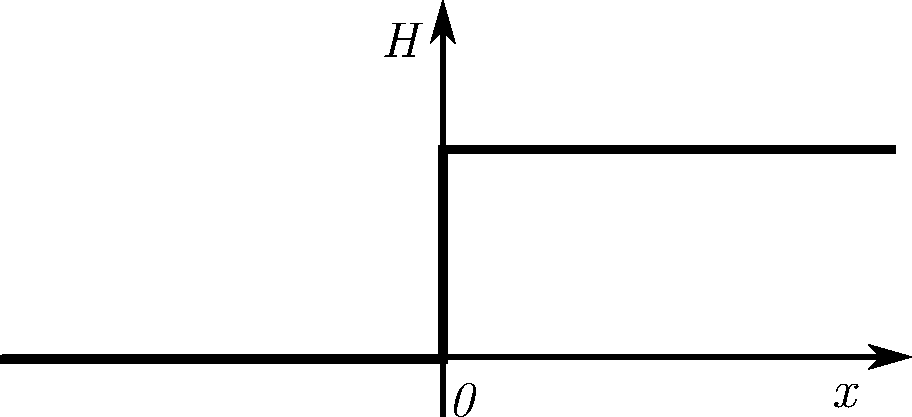
\includegraphics[width=0.5\textwidth]{heaviside.pdf}
	\caption{Gradino unitario.}
	\label{heaviside}
\end{figure}
\noindent
Infatti
\[
	\left< H', \phi \right>= - \left< H, \phi ' \right>
	=- \int_0^{\infty} \phi'(x) dx
	=- \left[ \phi (x) \right]^{+ \infty}_{0}
	= \phi(0)= \left< \delta, \phi \right>
\]
cio\`e
\[
	H'=\delta
\]
nel senso delle distribuzioni.
Si noti che la derivata di $H$ nel senso usuale \`e la funzione nulla definita
per $x \neq 0$.
\section{Considerazioni sulla soluzione fondamentale}
Torniamo a considerare la soluzione fondamentale
\[
	\Gamma_D(t,x)= \frac{1}{\sqrt{4D\pi t}}
	e^{-\left( x^2/4Dt \right)}
\]
che descrive l'evoluzione per $t>0$ della densit\`a lineare di una massa totale
$m=1$ inizialmente concentrata in $x=0$ al tempo $t=0$.
Se la massa \`e realizzata attraverso un grande numero $N$ di particelle poste
in $x=0$ per $t=0$, l'integrale di densit\`a normale (gaussiana)
\[
	\frac{1}{\sqrt{4 \pi D t}}\int_a^b
	e^{-\left( x^2/4Dt \right)} dx
\]
descrive la probabilit\`a che una di queste particelle si trovi al tempo $t$
nell'intervallo $[a,b]$, quindi la percentuale di particelle presenti in $[a,b]$
al tempo $t$.\\
Il dato iniziale
\[
	\Gamma_D(0,x)= \delta
\]
\`e altamente singolare: non \`e nemmeno descrivibile attraverso una funzione
per singolare che la si voglia pensare.
Eppure per ogni $t>0$ la soluzione \`e estremamente regolare: ha derivate
(usuali)
di ogni ordine e va rapidamente a $0$ per $x \to \pm \infty$ assieme a tutte
le proprie derivate.
Il processo di diffusione \`e quindi {\bf regolarizzante}.
Infine, istantaneamente ad un qualunque $t>0$ si ha $\Gamma_D(0,x)>0$ per ogni
$x$. Ci\`o significa che la massa si diffonde istantaneamente dal singolo punto
$x=0$ e tutto l'asse reale con {\bf velocit\`a di propagazione infinita}.
Questo a volte \`e un limite nell'applicazione del modello anche se
$\Gamma_D(0,x)$
\`e quasi nulla al di fuori dell'intervallo $[-2D, 2D]$ per $t<<1$ e
l'integrale in $dx$ su tale intervallo vale l'intera massa $m=1$ per gli
stessi tempi ``piccoli''.
\section{Problema di Cauchy omogeneo}
Risolviamo il sistema
\[
	\left\{
	\begin{array}{l}
		u_t= Du_{xx}\\
		u(0,x)= g(x)
	\end{array}
	\right.
	\substack{\displaystyle{\mathscr{F}} \\ \follows}
	\left\{
	\begin{array}{l}
		v_t= -D\lambda v\\
		v(0,\lambda)= \hat{g}(\lambda)
	\end{array}
	\right.
\]
\[
	v(t, \lambda)= c(\lambda)e^{-D\lambda^2t}
\]
\[
	v(0,t)= \hat{g}(\lambda)
\]
\[
	\Downarrow
\]
\[
	c(\lambda)= \hat{g}(\lambda)
\]
Trovando l'unica soluzione per $v$
\[
	v(t,\lambda)= \hat{g}(\lambda)e^{-D\lambda^2t}
\]
e antitrasformando ($\mathscr{F}^{-1}$)
\[
	u(t,x)= g(x) \circledast \Gamma_D(t,x)
\]
Dato che
\[
	\Gamma_D(t,x)=
	\frac{1}{\sqrt{4D\pi t}}
	e^{-\left( x^2/4Dt \right)}
\]
risultava essere la soluzione fondamentale, cio\`e con $g(x)=\delta(x)$,
la soluzione generica \`e composta dalla somma di tutti gli effetti elementari
\[
	u(t,x)= \frac{1}{\sqrt{4D\pi t}} \intR
	e^{\left( -(x-y)^2 / 4Dt \right)}
	g(y) dy
\]
\section{Problema di Cauchy non omogeneo}
Risolveremo il problema tramite la trasformata di Fourier.
Tale procedimento fornisce anche un risultato di unicit\`a della soluzione:
se la trasformata \`e univocamente determinata, tale \`e anche la soluzione.
\[
	\left\{
	\begin{array}{ll}
		u_t= Du_{xx}+ f & \text{con } f= f(t,x)\\
		u(0,x)= g(x)
	\end{array}
	\right.
\]
trasformando con Fourier
\[
	v(t,\lambda)= \intR e^{-i\lambda x} u(t,x) dx
\]
\[
	\left\{
	\begin{array}{l}
		v_t= -D\lambda^2 v+ \hat{f} \\
		v(0,\lambda)= \hat{g}(x)
	\end{array}
	\right.
\]
Consideriamo quindi
\[
	v_t + D \lambda^2 v =\hat{f}
\]
da cui, moltiplicando per il fattore integrante $e^{D\lambda^2 t}$
\[
	e^{D\lambda^2 t} v_t + e^{D\lambda^2 t} D \lambda^2 v
	=e^{D\lambda^2 t} \hat{f}
\]
\[
	\frac{d}{dt}\left(
	e^{D\lambda^2 t} v \right)
	= e^{D\lambda^2 t} \hat{f}
\]
\[
	e^{D\lambda^2 t} v
	= \int e^{D\lambda^2 t} \hat{f}(t, \lambda) dt
	+\underbracket{C(\lambda)}_{\mathclap{\text{Costanti rispetto a } t}}
\]
Dal teorema fondamentale del calcolo integrale
\[
	\int_0^t \frac{d}{d\tau}\left(
	e^{D\lambda^2 \tau} v(\tau, \lambda) \right) d\tau=
	e^{D\lambda^2 t} v(t, \lambda) - e^{D\lambda^2 0} v(0,\lambda)
\]
quindi si pu\`o scrivere
\[
	\int_0^t e^{D\lambda^2 \tau} \hat{f}(\tau, \lambda) d\tau
	= e^{D\lambda^2 t} v(t, \lambda) - e^{D\lambda^2 0} v(0,\lambda)
	= e^{D\lambda^2 t} v(t, \lambda) - v(0,\lambda)
\]
\[
	\int_0^t e^{D\lambda^2 \tau} \hat{f}(\tau, \lambda) d\tau
	+\hat{g}(\lambda)
	= e^{D\lambda^2 t} v(t, \lambda)
\]
\[
	v(t,\lambda)= e^{-D\lambda^2 t} +\hat{g}(\lambda)
	+ \int_0^t e^{-D\lambda^2 (t - \tau)} \hat{f}(\tau, \lambda) d\tau
\]
Antitrasformando, tenuto conto che
\[
	\hat{\Gamma}_D(t,\lambda)= e^{-D\lambda^2 t},
\]
si ottiene
\[
	u(t,x)= \underbracket{\Gamma_D(t,x)\circledast g(x)}_{u_1}+
	\underbracket{\int_0^t \Gamma_D(t-\tau, x)
	\circledast f(\tau, x) d\tau}_{u_2}
\]
perci\`o
\[
	u(t,x)= u_1(t,x)+ u_2(t,x)
\]
Analizzando le varie parti della soluzione, si nota che $u_1$ risolve
il problema omogeneo senza sorgente facendosi carico della situazione
iniziale; in particolare risolve il il problema
\[
	\left\{
	\begin{array}{l}
		u_t=Du_{xx} \\
		u(0,x)= g(x)
	\end{array}
	\right.
\]
Per quanto riguarda $u_2$, il termine
\[
	\Gamma_D(t-\tau, x)
	\circledast f(\tau, x)
\]
\`e uguale all'evoluzione al tempo $t$, dopo un tempo trascorso dall'istante
$\tau$ all'istante $t$ pari a $t-\tau$, di una densit\`a $f(\tau, x)$ immessa
sul sistema al tempo $\tau$. Si noti che la convoluzione contrassegnata con
$\circledast$ \`e rispetto alla variabile spaziale e non al tempo.\\
La soluzione $u_2$ risolve
\[
	\left\{
	\begin{array}{l}
		u_t=Du_{xx} +f \\
		u(0,x)= 0
	\end{array}
	\right.
\]
\subsection{\texorpdfstring
{Esercizio: Dimostrare che $u(0,x) \in L^2$, allora $u(t,x) \in L^2$}
{Esercizio: Dimostrare che se u(0,x) \`e a quadrato sommabile,
allora lo \`e anche u(t,x)}}
Dato il problema
\[
	\left\{
	\begin{array}{ll}
		u_t=Du_{xx} & t>0\\
		u(0,x)= g(x)
	\end{array}
	\right.
\]
\[
	E(t)= \frac{1}{2}\intR \left| u(t,x)\right|^2 dx
\]
Utilizzando il teorema di Parseval
\[
	\intR \left| u(t,x)\right|^2dx
	= \frac{1}{2\pi} \intR \left| v(t,\lambda) \right|^2 d\lambda
\]
Si noti che \`e stato considerato $u$ reale, perci\`o $u^2= |u|^2$.\\
Si \`e mostrato in precedenza che la soluzione $v(t,\lambda)$ (cio\`e la
trasformata di $u$) \`e
\[
	v(t,\lambda)= e^{-D\lambda^2 t} \hat{g}(\lambda)
\]
quindi
\[
	\left| v(t,\lambda) \right|^2 = e^{-2D\lambda^2 t}
	\left| \hat{g}(\lambda) \right|^2
\]
e immediatamente si osserva che al crescere del tempo $t$
la funzione decresce.\\
Riprendendo Parseval
\[
	\intR \left| u(t,x)\right|^2 dx= \frac{e^{-2D\lambda^2 t}}{2\pi}
	\intR \left| \hat{g}(\lambda) \right|^2 d\lambda
\]
in $t=0$
\[
	\intR \left| \hat{g}(\lambda) \right|^2 d\lambda=
	2\pi \intR \left| u(0,x)\right|^2 dx
\]
\[
	\intR \left| u(t,x)\right|^2 dx= e^{-2D\lambda^2 t}
	\intR \left| u(0,x)\right|^2 dx
\]
e per qualsiasi $t\geq 0$
\[
	\intR \left| u(t,x)\right|^2 dx \leq
	\intR \left| g(x) \right|^2 dx
\]
In conclusione
\[
	E(t)\leq E(0)
\]
Sfruttando il risultato appena illustrato si possono ottenere le stesse
conclusioni del caso finito, cio\`e l'unicit\`a e la dipendenza continua
dai dati secondo la norma $L^2$
\[
	\intR \left| u_1-u_2 \right|^2 dx
	\leq
	\intR \left| g_1 - g_2 \right|^2 dx
\]
